\subsection{Design}
This section describes the main aspects of the VFS Browser application. It shows
the implementation of the core interfaces and classes.

\subsubsection{GUI classes}\label{sec:guiClasses}
Figure \ref{fig:gui_classes} gives an overview of the main interfaces and
classes that were implemented for the GUI. The implementation followed the rules
of a MVC design dividing the aspects of Model View and Control to their
respective classes. According to the partition of MVC the classes were
partitioned into the packages \textit{model, view and controller}.

\begin{figure}[h!]
\centering
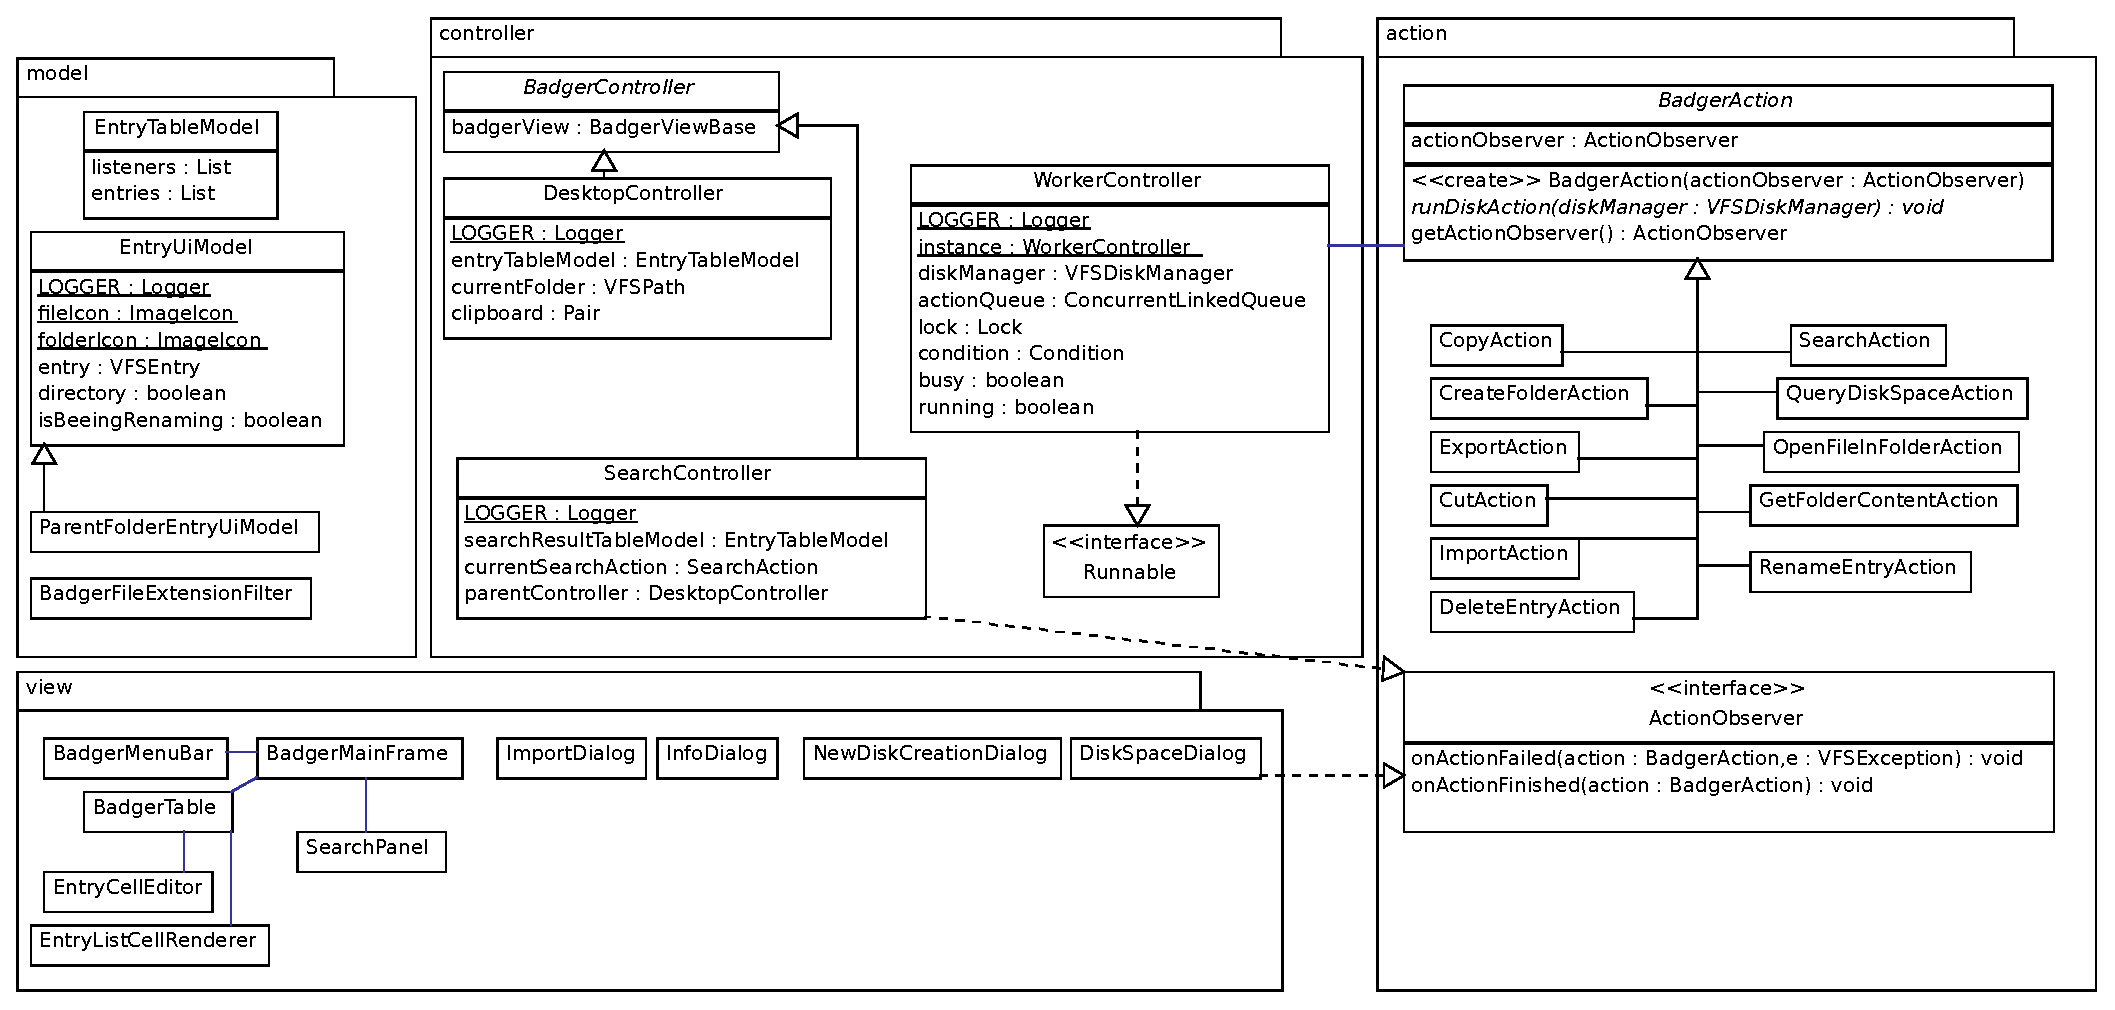
\includegraphics[width=1\textwidth]{figures/gui_classes.eps}
\caption{gui classes}
\label{fig:gui_classes}
\end{figure}


\subsubsection{Decoupling of GUI and working threads}
This section describes the way how the decoupling from GUI and working threads
was implemented. This decoupling made the GUI still responsive even though some
long running tasks like import or search would be running. All operations performed on the core components accessing the virtual disk file are encapsulated in subclasses of \textit{BadgerAction}. These \textit{BadgerActions} are then performed single theaded by the \textit{WorkerController}. By queuing these actions concurrent access to the virtual disk is prevented.

Figure
\ref{fig:decouple_threads} shows the sequence diagram of the example ``Import'':
The \textit{DesktopController} which lives in the GUI thread creates a new
\textit{ImportAction} that is enqueued in the \textit{WorkerController}'s action queue. It is worth to mention, that the
\textit{WorkerController} is a singleton, that has an \textit{instance} field. The
\textit{WorkerController} has a thread that works on a blocking queue and every
time it gets a \textit{BadgerAction} the thread wakes up and performs the action
on the VFS core API. After the API work is done (in this case the import of
files), the \textit{WorkerController} calls the corresponding
\textit{ActionObserver}, which is in most cases the \textit{DesktopController}
instance, so that the GUI can be updated. This design ensures single threaded
access on the VFS core API with keeping the GUI responsive.

\begin{figure}[h!]
\centering
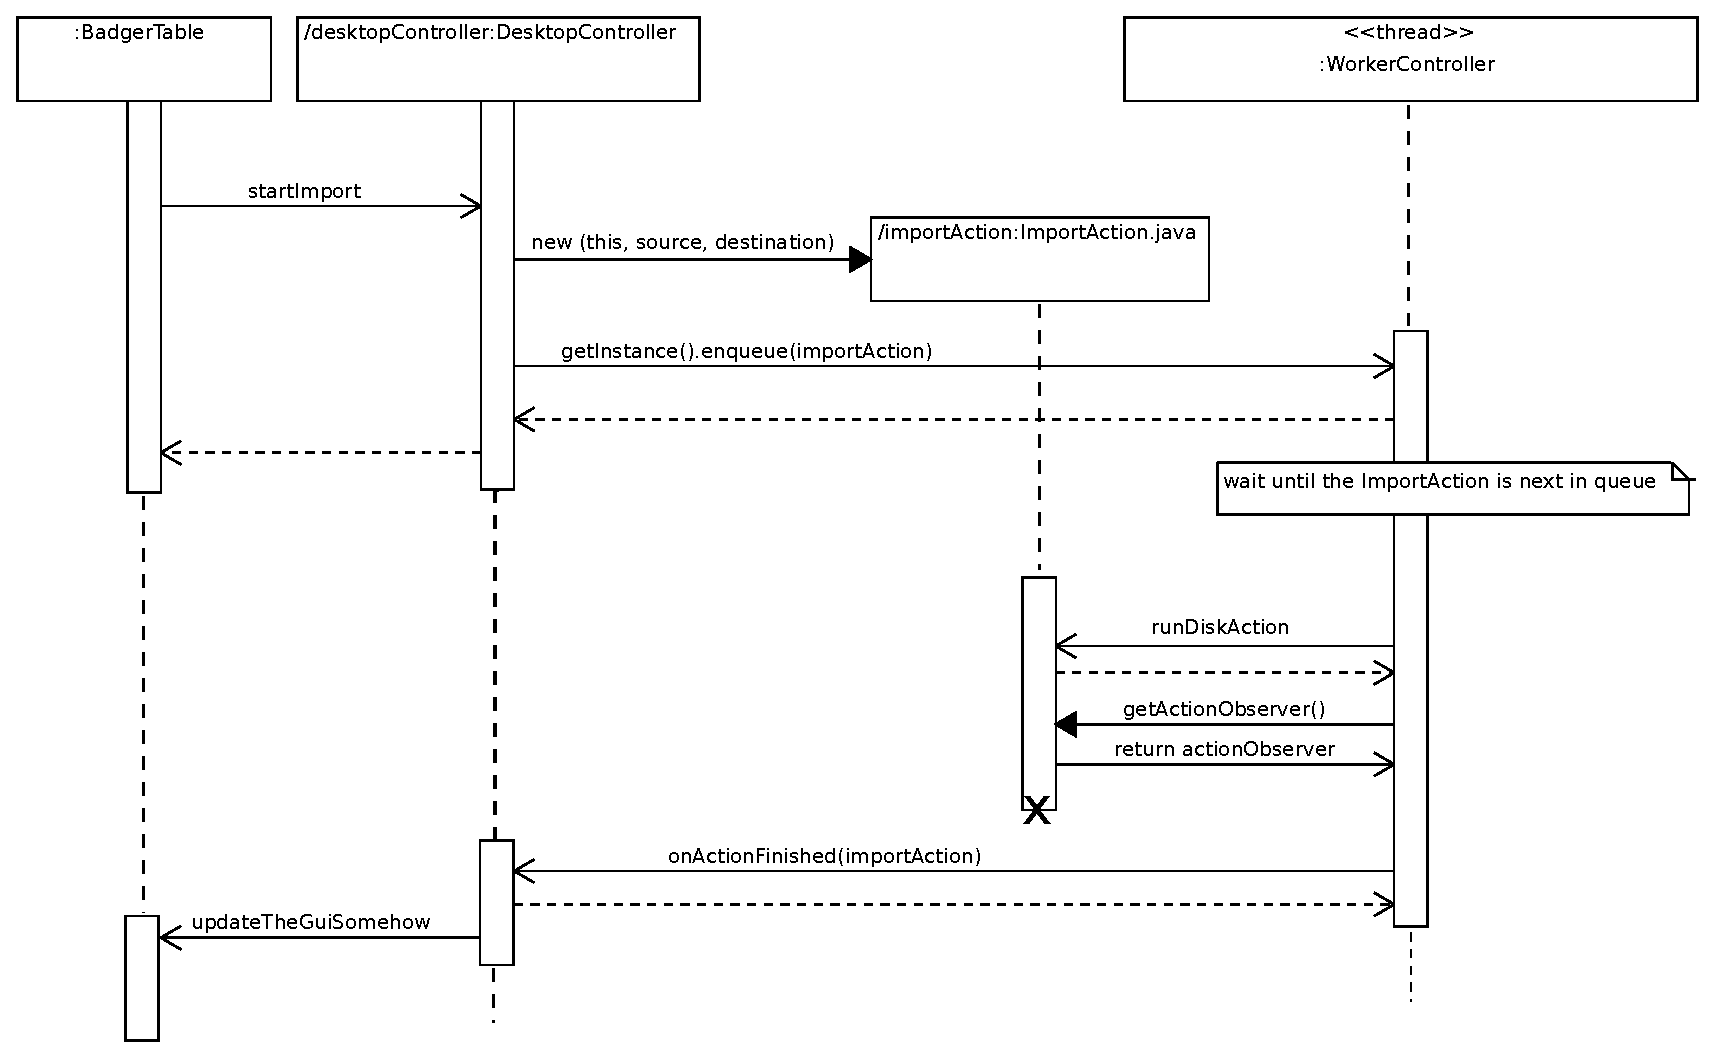
\includegraphics[width=1\textwidth]{figures/single_threaded_access.eps}
\caption{example of decoupling import from gui}
\label{fig:decouple_threads}
\end{figure}

Even when doing a seach the decoupling works pretty well: The
\textit{SearchAction} uses the VFS core's \textit{FindInFolderCallback} to
update the \textit{SearchController} every time finds an entry. Upon such an
update, the \textit{SearchController} updates the GUI.

\subsubsection{Search}
Searching files can be done in a separate Panel: After entering the search
string one is allowed to switch several flags like ``case sensitive'' or
``search subfolder'' and one can change the search folder. As mentioned before ? and * are supported as wildcards.

Search can be canceled on the gui at any time. However the search routine performed on the core checks for cancelation only once walking through a directory (which should be often enough).

A double click (or keyboard enter) on a search result stops the current search and opens the containing folder in the browsing window.

\subsubsection{Keyboard and Mouse support}
One can navigate the list of entries by double clicking folders. The parent
folder can be accessed by double clicking ``..''. By right clicking on an entry
the user gets a menu depending on wheter she clicked on an file, folder or the empty
space. The right click in empty space reveals the same menu entries as the right
click on the parent folder. The only difference between file and folder menus
are the ``new folder'', ``paste'' and ``import'' actions, that are not allowed
on files.

The user is also allowed to select several files and folders from the list and
can then perform cut/copy or export on the selected items. 


\paragraph{Keyboard Shortcuts}
For keyboard wizards there are several keyboard shortcuts for doing the actions
on the selected entries. They keep to the general standards like F2 for renaming
or Ctrl+C for copy. The menus indicate the available shortcuts.
\paragraph{Drag \& Drop}
For doing quick import, the user is allowed to drag\&drop files or folders from
the host file system to the current folder. On doing such an import a small
progress window is displayed, that show how much of the task is already
finished, and how much has yet to be done.
